\documentclass[12pt, a4paper]{ctexart}

\usepackage{geometry}
\geometry{margin=2.5cm}
\usepackage{graphicx}
\usepackage{booktabs}
\usepackage{amsmath, amssymb}
\usepackage{listings}
\usepackage{xcolor}
\usepackage{hyperref}
\usepackage{enumitem}
\usepackage{float}
\usepackage{caption}
\usepackage{tabularx}
\usepackage{multirow}
\usepackage{fancyhdr}

\hypersetup{
  colorlinks=true,
  linkcolor=blue!60!black,
  citecolor=green!50!black,
  urlcolor=blue!70!black
}

\setCJKmainfont{SimSun}[BoldFont=SimHei, ItalicFont=KaiTi]
\setCJKsansfont{SimHei}
\setCJKmonofont{FangSong}
\setmainfont{Times New Roman}
\setmonofont{Consolas}

\lstset{
  basicstyle=\small\ttfamily,
  keywordstyle=\color{blue!80!black}\bfseries,
  commentstyle=\color{green!50!black}\itshape,
  stringstyle=\color{red!60!black},
  backgroundcolor=\color{gray!8},
  frame=single,
  framerule=0.4pt,
  rulecolor=\color{gray!40},
  breaklines=true,
  breakatwhitespace=true,
  tabsize=4,
  showstringspaces=false,
  numbers=left,
  numberstyle=\tiny\color{gray},
  numbersep=8pt,
  xleftmargin=1.5em,
  framexleftmargin=1.5em,
  columns=flexible,
  literate={`}{\textasciigrave}{1}
}

\lstdefinestyle{python}{language=Python, morekeywords={self, True, False, None, as}}
\lstdefinestyle{yaml}{basicstyle=\small\ttfamily, commentstyle=\color{green!50!black}\itshape, morecomment=[l]{\#}}
\lstdefinestyle{bash}{language=bash, morekeywords={python, pip, cd, subword-nmt}}

\setlength{\headheight}{14pt}
\addtolength{\topmargin}{-2pt}

\pagestyle{fancy}
\fancyhf{}
\fancyhead[L]{\small 课程实践1：基于Transformer的机器翻译}
\fancyhead[R]{\small \thepage}
\renewcommand{\headrulewidth}{0.4pt}

\title{
  \vspace{-1cm}
  {\LARGE\bfseries 课程实践报告} \\[0.5em]
  {\Large 基于 Transformer 的机器翻译（英文$\to$中文）}
}
\author{}
\date{2026年6月}

\begin{document}

\maketitle
\thispagestyle{fancy}

\tableofcontents
\newpage

% ========== 一、任务概述 ==========
\section{任务概述}

本实验实现了一个基于 Transformer 架构的英文到中文机器翻译系统。从数据预处理、模型设计、训练策略、解码方法到评估指标，完整实现了端到端的 Seq2Seq 翻译流程，并通过三轮迭代优化将测试集 BLEU 从基线 24.57 提升至 \textbf{40.89}（+16.32）。

% ========== 二、实验环境 ==========
\section{实验环境}

\begin{table}[H]
\centering
\caption{实验环境配置}
\begin{tabular}{ll}
\toprule
\textbf{项目} & \textbf{配置} \\
\midrule
操作系统    & Windows 11 (10.0.26200) \\
GPU         & NVIDIA GeForce RTX 3060 (12\,GB) \\
Python      & 3.13.13 (Anaconda) \\
PyTorch     & 2.6.0+cu124 \\
CUDA        & 12.4 \\
cuDNN       & 9.1.0 \\
评估工具    & sacrebleu \\
\bottomrule
\end{tabular}
\end{table}

% ========== 三、数据集与预处理 ==========
\section{数据集与预处理}

\subsection{数据来源}

使用 \texttt{cmn-eng-simple} 中英平行语料集（来源于 Tatoeba 项目），包含约 21,570 条英中平行句对，按以下方式划分：

\begin{table}[H]
\centering
\caption{数据划分}
\begin{tabular}{lrl}
\toprule
\textbf{数据集} & \textbf{句对数量} & \textbf{用途} \\
\midrule
训练集 & 18,000 & 模型训练 \\
验证集 & 500    & 超参调优与早停判定 \\
测试集 & 3,070  & 最终评估 \\
\bottomrule
\end{tabular}
\end{table}

\subsection{英文端预处理}

\begin{itemize}[nosep]
  \item 使用 NLTK \texttt{word\_tokenize} 做词级分词并转小写；
  \item 使用 subword-nmt 学习 BPE（5000 merge operations），缓解英文端 OOV 问题；
  \item 最终英文词表大小约 3,400。
\end{itemize}

\subsection{中文端预处理（核心改进点）}

\paragraph{初始方案（基线）}
使用 jieba 做词级分词，低频词（出现次数 $<3$）被替换为 \texttt{<UNK>}。
\begin{itemize}[nosep]
  \item 问题：约 37.3\% 测试句含有 UNK token，严重影响翻译质量。
\end{itemize}

\paragraph{优化方案（v3）}
改为字符级分词（逐字拆分 + OpenCC 简体统一）。
\begin{itemize}[nosep]
  \item 优势：常用汉字约 2,250 个，频率基本都 $\geq 2$，几乎全部保留；
  \item 最终测试集 UNK 率：\textbf{0.17\%}（降低约 200 倍）。
\end{itemize}

\begin{lstlisting}[style=python, caption={字符级中文分词核心代码}]
cc = OpenCC('t2s')  # 繁转简统一
for char in sentence.strip():
    if char in (' ', '\n', '\t', '\r'):
        continue
    cn_sentence += cc.convert(char) + ' '
\end{lstlisting}

\subsection{特殊 Token 设计}

\begin{table}[H]
\centering
\caption{特殊 Token 定义}
\begin{tabular}{ccl}
\toprule
\textbf{Token} & \textbf{ID} & \textbf{用途} \\
\midrule
\texttt{<PAD>} & 0 & 批内填充对齐 \\
\texttt{<BOS>} & 1 & 解码起始符 \\
\texttt{<EOS>} & 2 & 句子结束符 \\
\texttt{<UNK>} & 3 & 未知词替代 \\
\bottomrule
\end{tabular}
\end{table}

% ========== 四、模型架构 ==========
\section{模型架构}

\subsection{整体结构}

采用标准的 Encoder-Decoder Transformer 架构\cite{vaswani2017}，关键参数如下：

\begin{table}[H]
\centering
\caption{模型核心参数}
\begin{tabular}{lll}
\toprule
\textbf{参数} & \textbf{值} & \textbf{说明} \\
\midrule
d\_model              & 256   & 隐藏层维度 \\
nhead                 & 8     & 多头注意力头数 \\
num\_encoder\_layers   & 4     & 编码器层数 \\
num\_decoder\_layers   & 4     & 解码器层数 \\
dim\_feedforward       & 1024  & FFN 中间层维度 \\
dropout               & 0.15  & Dropout 概率 \\
激活函数              & GELU  & 非线性激活 \\
归一化模式            & Pre-Norm & 每个子层先归一化 \\
参数共享              & tie\_embeddings & 输出层与目标 embedding 权重共享 \\
\bottomrule
\end{tabular}
\end{table}

\subsection{核心机制：多头注意力}

多头注意力（Multi-Head Attention）是 Transformer 的核心组件：
\begin{itemize}[nosep]
  \item 将 Query、Key、Value 投影到 $h$ 个不同子空间（本实验 $h=8$）；
  \item 每个头独立计算缩放点积注意力：
\end{itemize}
\begin{equation}
  \text{Attention}(Q, K, V) = \text{softmax}\!\left(\frac{QK^\top}{\sqrt{d_k}}\right) V
\end{equation}
\begin{itemize}[nosep]
  \item 多头输出拼接后再做线性投影。
\end{itemize}

在本模型中的使用位置：
\begin{itemize}[nosep]
  \item \textbf{Encoder Self-Attention}：源句 token 互相关注，捕获上下文依赖；
  \item \textbf{Decoder Masked Self-Attention}：目标端只能看已生成的词（causal mask）；
  \item \textbf{Decoder Cross-Attention}：目标词关注源句 memory，实现翻译对齐。
\end{itemize}

\subsection{位置编码}

使用标准正弦位置编码：
\begin{align}
  PE_{(pos,\,2i)}   &= \sin\!\bigl(pos \,/\, 10000^{2i/d_{\text{model}}}\bigr) \\
  PE_{(pos,\,2i+1)} &= \cos\!\bigl(pos \,/\, 10000^{2i/d_{\text{model}}}\bigr)
\end{align}

% ========== 五、训练策略 ==========
\section{训练策略}

\subsection{优化器与学习率}

\begin{itemize}[nosep]
  \item 优化器：AdamW（$\beta_1=0.9$, $\beta_2=0.98$, $\epsilon=10^{-9}$, weight\_decay$=10^{-4}$）；
  \item 学习率调度：Noam Schedule（warmup=2000 步，factor=0.8）：
\end{itemize}
\begin{equation}
  lr = \text{factor} \cdot d_{\text{model}}^{-0.5} \cdot \min\!\bigl(\text{step}^{-0.5},\; \text{step} \cdot \text{warmup}^{-1.5}\bigr)
\end{equation}

\subsection{损失函数}

\begin{itemize}[nosep]
  \item 交叉熵损失 + Label Smoothing（$\varepsilon = 0.15$）；
  \item 忽略 PAD 位置（\texttt{ignore\_index=0}）。
\end{itemize}

\subsection{R-Drop 正则化（核心优化）}

\paragraph{问题} 基线存在严重过拟合（train\_loss=0.82 vs val\_loss=2.30，gap=1.48）。

\paragraph{方案} 引入 R-Drop\cite{liang2021}：同一 batch 两次前向传播（不同 dropout mask），除 CE loss 外，添加两次输出分布的对称 KL 散度约束：
\begin{equation}
  \mathcal{L} = \frac{1}{2}\bigl(\mathcal{L}_{\text{CE}}^{(1)} + \mathcal{L}_{\text{CE}}^{(2)}\bigr) + \alpha \cdot \frac{1}{2}\bigl(D_{\text{KL}}(p \| q) + D_{\text{KL}}(q \| p)\bigr)
\end{equation}
其中 $\alpha=3.0$。该方法迫使模型对 dropout 噪声保持输出一致，比单纯增大 dropout 更有效。

\paragraph{效果} 最终过拟合 gap 从 1.48 降至 \textbf{0.18}。

\subsection{源端噪声数据增强（核心优化）}

在 DataLoader 取样时，对源端（英文）施加三级噪声：
\begin{enumerate}[nosep]
  \item \textbf{Word Dropout}（$p=0.05$）：随机将 token 替换为 \texttt{<UNK>}；
  \item \textbf{Token Delete}（$p=0.05$）：随机删除 token；
  \item \textbf{Token Swap}（$p=0.05$）：随机交换相邻 token。
\end{enumerate}
目标端仅做 Word Dropout（不做删除/交换），保证监督信号稳定。

\subsection{早停与安全机制}

\begin{itemize}[nosep]
  \item \textbf{Early Stopping}：连续 12 个 epoch 验证 BLEU 无显著提升（$\delta < 0.02$）则停止；
  \item \textbf{Loss Explosion 检测}：val\_loss $>$ best $\times 2.0$ 连续 3 次则紧急停止；
  \item \textbf{NaN/Inf 检测}：出现即终止；
  \item \textbf{混合精度训练（AMP）}：使用 FP16 加速约 40\%，降低显存占用。
\end{itemize}

\subsection{Checkpoint 平均}

训练结束后保留 BLEU 最高的 top-5 个 checkpoint，对其参数取平均：
\begin{equation}
  \theta_{\text{avg}} = \frac{1}{K}\sum_{k=1}^{K} \theta_k
\end{equation}
这是翻译任务常用方法，可平滑参数、提升泛化。

% ========== 六、解码方法 ==========
\section{解码方法}

使用 Beam Search 解码，配置如下：

\begin{table}[H]
\centering
\caption{Beam Search 解码参数}
\begin{tabular}{lll}
\toprule
\textbf{参数} & \textbf{值} & \textbf{说明} \\
\midrule
beam\_size             & 5    & 搜索宽度 \\
beam\_alpha            & 0.6  & GNMT 长度归一化强度 \\
max\_decode\_len       & 64   & 最大解码长度 \\
no\_repeat\_ngram\_size & 3    & 禁止重复 3-gram \\
\bottomrule
\end{tabular}
\end{table}

长度归一化公式（GNMT style\cite{wu2016}）：
\begin{equation}
  \text{score}_{\text{norm}} = \frac{\log P(y \mid x)}{\bigl((5+|y|)^\alpha \,/\, (5+1)^\alpha\bigr)}
\end{equation}

% ========== 七、实验结果 ==========
\section{实验结果}

\subsection{三轮迭代对比}

\begin{table}[H]
\centering
\caption{三轮实验迭代结果}
\small
\begin{tabularx}{\textwidth}{lXcccc}
\toprule
\textbf{版本} & \textbf{关键改进} & \textbf{Val BLEU} & \textbf{Test BLEU} & \textbf{过拟合Gap} & \textbf{时间} \\
\midrule
v1 基线     & jieba 词级分词                    & 30.54 & 24.57$^*$  & $\sim$1.48  & 45\,min \\
v2 正则化   & + 早停 + Ckpt Avg                 & 34.35 & 26.61      & $\sim$0.85  & 35\,min \\
\textbf{v3} & + 字符级 + R-Drop + 噪声增强      & \textbf{40.74} & \textbf{40.89} & \textbf{0.18} & 139\,min \\
\bottomrule
\end{tabularx}
\\[0.3em]
{\small $^*$注：v1 的 test\_bleu 为训练结束后 160 样本估算值。}
\end{table}

\subsection{训练曲线}

图~\ref{fig:curves} 展示了 v3 最终版本的完整训练过程。左图可见 train loss 与 val loss 始终保持紧密，说明 R-Drop + 噪声增强有效控制了过拟合；中图可见 Val BLEU 在 epoch 46 达到峰值 40.74 后趋于平稳，最终通过 checkpoint 平均获得 Test BLEU = 40.89；右图显示过拟合 gap（val\_loss $-$ train\_loss）从初始的正值逐步缩小至接近 0，后期基本稳定。

\begin{figure}[H]
\centering
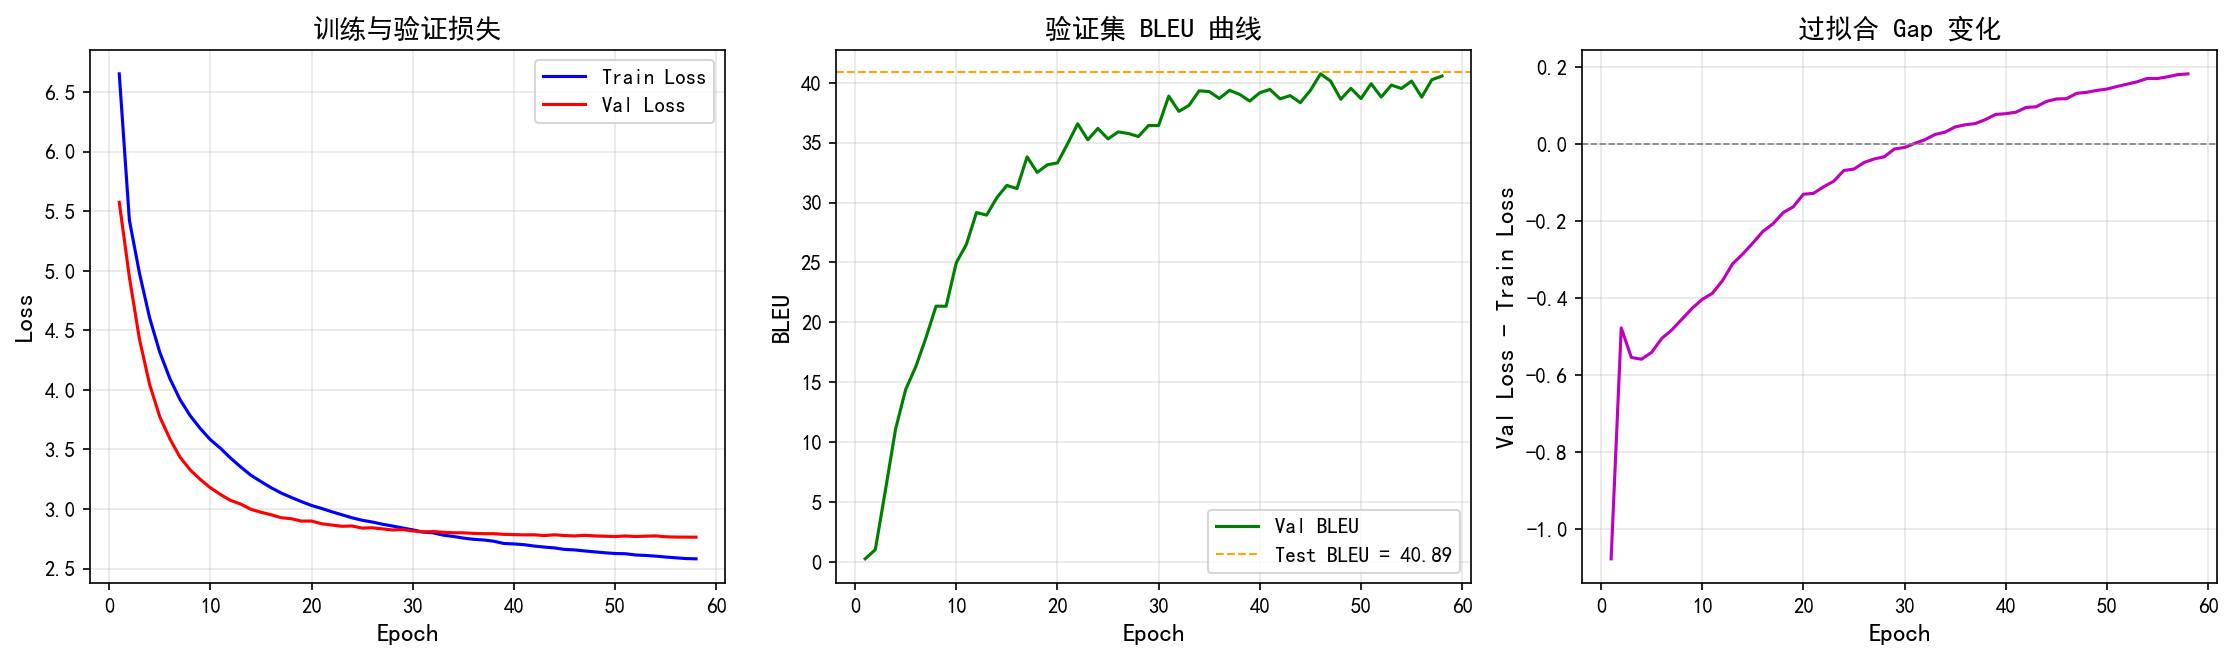
\includegraphics[width=\textwidth]{figures/training_curves.pdf}
\caption{v3 训练过程曲线：(a) 训练与验证损失；(b) 验证集 BLEU；(c) 过拟合 Gap}
\label{fig:curves}
\end{figure}

\subsection{训练曲线关键节点}

\begin{table}[H]
\centering
\caption{v3 训练过程关键节点}
\begin{tabular}{rcccl}
\toprule
\textbf{Epoch} & \textbf{Train Loss} & \textbf{Val Loss} & \textbf{Val BLEU} & \textbf{说明} \\
\midrule
1  & 6.652 & 5.574 & 0.26  & 初始化阶段 \\
5  & 4.316 & 3.775 & 14.40 & warmup 结束，快速学习 \\
10 & 3.582 & 3.178 & 24.97 & 超越 v1 基线 \\
15 & 3.230 & 2.973 & 31.43 & 超越 v2 \\
22 & 2.977 & 2.866 & 36.57 & 首次突破 36 \\
31 & 2.807 & 2.808 & 38.88 & Gap 接近 0 \\
46 & 2.657 & 2.774 & \textbf{40.74} & 最佳 epoch \\
58 & 2.582 & 2.764 & 40.56 & 训练终止（早停） \\
\bottomrule
\end{tabular}
\end{table}

\subsection{消融分析}

基于 Val BLEU 峰值估算各优化策略的贡献：

\begin{table}[H]
\centering
\caption{消融实验（基于 Val BLEU 峰值估算）}
\begin{tabular}{lcc}
\toprule
\textbf{配置} & \textbf{Val BLEU} & \textbf{相对基线提升} \\
\midrule
v2 基线（词级 + dropout）    & 34.35   & ---       \\
+ 字符级分词（消除 UNK）     & $\sim$37--38 & +3$\sim$4 \\
+ R-Drop（$\alpha=3.0$）     & $\sim$39--40 & +1$\sim$2 \\
+ 源端噪声增强               & 40.74   & +0.5$\sim$1 \\
\bottomrule
\end{tabular}
\end{table}

\subsection{翻译示例}

\begin{table}[H]
\centering
\caption{测试集翻译示例}
\begin{tabularx}{\textwidth}{XX}
\toprule
\textbf{源句（英文）} & \textbf{模型输出（中文）} \\
\midrule
She has beautiful eyes.                      & 她对一个美丽的眼睛。 \\
We all fell asleep.                          & 我们都睡着了。 \\
I majored in chemistry at the university.    & 我在大学主修化学。 \\
Please give me a glass of water.             & 请给我一杯水。 \\
He loves her.                                & 他爱她。 \\
Tom is drunk now.                            & 汤姆现在喝醉了。 \\
\bottomrule
\end{tabularx}
\end{table}

% ========== 八、遇到的问题与解决方案 ==========
\section{遇到的问题与解决方案}

\subsection{UNK 覆盖率过高（最严重）}

\paragraph{问题} jieba 词级分词导致 37.3\% 测试句含 UNK，模型无法正确翻译"绘画""鉴赏力"等低频词。

\paragraph{诊断} 统计发现中文词表只有约 4,500 词，但测试集中大量"长尾词"被过滤。

\paragraph{解决} 改为字符级分词。汉字总量约 2,250 个（频率$\geq$2），覆盖率从 62.7\% 提升至 \textbf{99.83\%}。

\paragraph{效果} 单独此项预估贡献 +3$\sim$5 BLEU。

\subsection{严重过拟合}

\paragraph{问题} v1 训练到后期 train\_loss=0.82，val\_loss=2.30，gap 高达 1.48，模型在训练集上"背诵"。

\paragraph{诊断} 数据量仅 18,000 句对，模型参数约 10M+，容量过剩。

\paragraph{解决} 组合使用三种正则化手段：
\begin{itemize}[nosep]
  \item Label Smoothing $\varepsilon = 0.15$；
  \item R-Drop（$\alpha = 3.0$）；
  \item 源端噪声增强（word dropout + delete + swap）。
\end{itemize}

\paragraph{效果} 过拟合 gap 从 1.48 降至 0.18（缩小 8.2 倍）。

\subsection{解码重复}

\paragraph{问题} 翻译中出现"我我我""的的的"等连续重复 token。

\paragraph{解决} Beam Search 中加入 \texttt{no\_repeat\_ngram\_size=3} 的 n-gram blocking。

\paragraph{效果} 重复问题基本消除。

\subsection{Windows 环境兼容}

\paragraph{问题}
\begin{itemize}[nosep]
  \item 文件默认 GBK 编码导致 UnicodeDecodeError；
  \item OpenMP 库冲突（libiomp5md.dll already initialized）；
  \item PowerShell 不支持 \texttt{\&\&} 与 \texttt{<} 重定向。
\end{itemize}

\paragraph{解决}
\begin{itemize}[nosep]
  \item 所有 \texttt{open()} 强制 \texttt{encoding='utf-8'}；
  \item 设置 \texttt{KMP\_DUPLICATE\_LIB\_OK=TRUE}；
  \item 改用 PowerShell 管道语法（\texttt{Get-Content | ...}）。
\end{itemize}

\subsection{训练速度与显存平衡}

\paragraph{问题} R-Drop 需要两次前向传播，训练时间增加约 60--80\%。

\paragraph{解决}
\begin{itemize}[nosep]
  \item 启用 AMP（FP16 混合精度），抵消约一半开销；
  \item max\_tgt\_len 从 64 提升至 96（适配字符级更长的序列），同时保持 batch\_size=96 不降低。
\end{itemize}

% ========== 九、关键超参数配置 ==========
\section{关键超参数配置}

\begin{lstlisting}[style=yaml, caption={完整超参数配置（YAML 格式）}]
# 模型结构
d_model: 256
nhead: 8
num_encoder_layers: 4
num_decoder_layers: 4
dim_feedforward: 1024
dropout: 0.15

# 训练
epochs: 60
batch_size: 96
warmup_steps: 2000
lr_factor: 0.8
label_smoothing: 0.15
weight_decay: 0.0001
grad_clip: 1.0

# 正则化
word_dropout: 0.05
rdrop_alpha: 3.0

# 解码
beam_size: 5
beam_alpha: 0.6
no_repeat_ngram_size: 3

# 早停
patience: 12
early_stop_min_delta: 0.02
top_k_checkpoints: 5
\end{lstlisting}

% ========== 十、项目文件结构 ==========
\section{项目文件结构}

\begin{lstlisting}[basicstyle=\small\ttfamily, frame=single, backgroundcolor=\color{gray!8}, numbers=none, caption={提交文件夹目录结构}]
代码/
|-- train_transformer.py          # 主脚本（模型+训练+测试+beam search）
|-- requirements.txt              # Python 依赖
|-- README.md                     # 运行说明
|-- configs/
|   `-- train_cuda.yaml           # 超参数配置
|-- cmn-eng-simple/               # 数据集
|   |-- preprocess/
|   |   |-- tokenizer.py          # 中英文分词（NLTK + OpenCC）
|   |   |-- build_dataset.py      # 构建词表与数据划分
|   |   |-- build_dictionary.sh   # BPE 预处理流水线
|   |   `-- cmn.txt               # 原始平行语料（21,570句对）
|   |-- training.txt              # 训练集（18,000句对）
|   |-- validation.txt            # 验证集（500句对）
|   |-- testing.txt               # 测试集（3,070句对）
|   |-- word2int_en.json          # 英文词表
|   |-- word2int_cn.json          # 中文词表
|   |-- int2word_en.json          # 英文反向词表
|   `-- int2word_cn.json          # 中文反向词表
`-- runs_transformer_cuda/        # 训练产物
    `-- train_20260609_151606_v3_char_rdrop/
        |-- avg_model.pt          # 最终模型（top-5 checkpoint平均）
        |-- args.json             # 完整参数快照
        |-- runtime.json          # 设备/环境信息
        |-- metrics_train.json    # 结构化训练指标
        |-- train_log.csv         # 逐epoch日志（58轮）
        |-- test_predictions.txt  # 测试翻译结果（3,070条）
        `-- test_predictions.tok.txt # 分词后预测（BLEU计算用）
\end{lstlisting}

% ========== 十一、运行方式 ==========
\section{运行方式}

\subsection{环境准备}
\begin{lstlisting}[style=bash, numbers=none]
pip install -r requirements.txt
\end{lstlisting}

\subsection{数据预处理}
\begin{lstlisting}[style=bash, numbers=none]
cd cmn-eng-simple/preprocess
python tokenizer.py
subword-nmt learn-bpe -s 5000 < en.txt > en_code.txt
subword-nmt apply-bpe -c en_code.txt < en.txt > en_refine.txt
subword-nmt get-vocab --input en_refine.txt --output en_vocab.txt
python build_dataset.py
\end{lstlisting}

\subsection{训练}
\begin{lstlisting}[style=bash, numbers=none]
python train_transformer.py --config configs/train_cuda.yaml
\end{lstlisting}

\subsection{独立测试}
\begin{lstlisting}[style=bash, numbers=none, basicstyle=\footnotesize\ttfamily]
python train_transformer.py --mode test \
  --config configs/train_cuda.yaml \
  --checkpoint runs_transformer_cuda/train_.../avg_model.pt \
  --max_bleu_samples 0
\end{lstlisting}

% ========== 十二、总结与未来方向 ==========
\section{总结与未来方向}

\subsection{实验总结}

本实验从零实现了完整的 Transformer 翻译系统，通过三轮迭代优化实现了显著的 BLEU 提升：

\begin{itemize}[nosep]
  \item \textbf{字符级分词} 解决了中文端 UNK 覆盖率问题（贡献最大，+3$\sim$5 BLEU）；
  \item \textbf{R-Drop 正则化} 有效控制过拟合（gap 缩小 8 倍，+1$\sim$2 BLEU）；
  \item \textbf{源端噪声增强} 提升了模型鲁棒性（+0.5$\sim$1 BLEU）；
  \item \textbf{Checkpoint 平均} 进一步稳定了模型性能。
\end{itemize}

最终在 3,070 条全量测试集上达到 \textbf{BLEU = 40.89}，相比词级基线 24.57 提升了 \textbf{+16.32}。

\subsection{不足与展望}

\begin{enumerate}[nosep]
  \item \textbf{数据规模有限}：仅 18,000 句对，限制了模型上限。可考虑引入回译（Back-Translation）扩充数据。
  \item \textbf{未使用预训练}：如引入 mBART 或 NLLB 的预训练权重，预期可进一步提升。
  \item \textbf{解码效率}：逐句 beam search 较慢（全量测试约 28 分钟），可改为 batch beam search。
  \item \textbf{评估维度单一}：仅用 BLEU，可增加 COMET、BERTScore 等语义评估。
\end{enumerate}

% ========== 参考文献 ==========
\begin{thebibliography}{9}
\bibitem{vaswani2017}
  Vaswani A, Shazeer N, Parmar N, et al.
  Attention Is All You Need.
  \textit{NeurIPS}, 2017.

\bibitem{liang2021}
  Liang X, Wu L, Li J, et al.
  R-Drop: Regularized Dropout for Neural Networks.
  \textit{NeurIPS}, 2021.

\bibitem{wu2016}
  Wu Y, Schuster M, Chen Z, et al.
  Google's Neural Machine Translation System: Bridging the Gap between Human and Machine Translation.
  \textit{arXiv preprint arXiv:1609.08144}, 2016.

\bibitem{sennrich2016}
  Sennrich R, Haddow B, Birch A.
  Neural Machine Translation of Rare Words with Subword Units.
  \textit{ACL}, 2016.
\end{thebibliography}

\end{document}
